\section*{Introduction} 
While not a reduction problem but instead a variant of the original Maximum Matching Problem, we can use the Stable Marriage Problem to better understand the nature and time complexity of the original problem. Through the use of matching people with relationships to one another, we already have a much more intuitive example of the original problem. By increasing the number of non-overlapping sets, relationships get increasingly more complex to map, growing from P class to NP-complete by simply going from bipartite to d-partite graphs. In this case, we consider the bipartite version to be the original problem proposed by Gale and Shapley and the 3D Stable Marriage Problem variant to be the d-partite variant. It is also by using stable matchings that we can find a max-matching, unless we use a Stable Marriage variant that specifically omits this property. 

This section summarizes the problem structure and several algorithms presented in Dan Gusfield and Robert W. Irving's book "The Stable Marriage Problem." It covers foundational knowledge necessary to understand the nature and complexity of the problem. Additionally, it surveys recent papers on the topic, illustrating how the problem and its accompanying algorithms has developed since the book's release in 1989. The paper examines the Gale-Shapley algorithm \cite{galeshapley} alongside several other relevant algorithms that have emerged since then.  

We’ll break down the key structure and algorithms presented in Dan Gusfield and Robert W. Irving’s work, "The Stable Marriage Problem." The goal here is to provide a solid understanding of the problem’s core concepts, particularly how stability and preferences interact within the context of algorithmic solutions like the well-known Gale-Shapley algorithm. After laying that groundwork, we’ll dive into a survey of relevant papers that have been published after the book’s release in 1989. These papers showcase the evolution of the problem, introducing new angles and improvements to the algorithms initially discussed. This includes updates on the theoretical complexity, practical applications, and how researchers have expanded upon the stable marriage framework in various ways.

\section*{Definitions}
The following section covers the definitions from the Gusfield and Irving book that are essential when understanding the Stable Marriage Problem (SMP) and its variants. This section serves as a reference since these terms will be used frequently in this section.
\begin{itemize}
    \item \textbf{Stable Matching}: A matching is called \emph{stable} if there are no two people, one from each side of the marriage problem, who would both prefer each other over their current partners. In other words, there are no \emph{blocking pairs}. Stability ensures that no person has the incentive to deviate from the matching.
    
    \item \textbf{Preference Lists}: Each individual in the SMP has a strict ordering of the members of the opposite group, ranking them based on preference. These rankings are used to determine which matchings are stable. Preference lists are central to the algorithmic process for finding stable matchings.
    
    \item \textbf{Unacceptable Partners}: In some variations of the SMP, an individual may consider certain members of the opposite group as \emph{unacceptable}. In such cases, they would rather remain unmatched than be paired with an unacceptable partner. These unacceptable partners are omitted from the individual’s preference list or at a position in the list where the agent would receive negative utility from being matched with them.
    
    \item \textbf{Indifference}: This refers to situations where an individual does not have a strict preference between two or more potential partners. Indifference leads to \emph{ties} in preference lists, complicating the stability conditions and algorithms used to find a stable matching. In the basic SMP, preference lists are assumed to be strict, but variations of the problem allow for the indifference property.
    
    \item \textbf{Blocking Pair}: A pair of individuals form a \emph{blocking pair} if they prefer each other over their current partners in a matching. The existence of any blocking pair makes a matching unstable. Blocking pairs only exist in the bipartite graph version of the problem. Thus, stability is defined as the absence of blocking pairs.
    
    \item \textbf{Optimality}: In the SMP, \emph{optimality} refers to a solution where one side of the matching get the best possible partner they could have in any stable matching. For instance, in the \emph{man-optimal} stable matching, each man is matched with the best partner they can get, considering stability.
    
    \item \textbf{Pessimality}: The opposite of optimality. In a \emph{man-pessimal} stable matching, each man is paired with the worst partner they could have in any stable matching. The pessimal matching is still stable but represents the least favorable outcome for one side.
    
    \item \textbf{Regret}: The \emph{regret} of an individual in a stable matching is defined as the ranking of their partner in their preference list. Lower-ranked partners lead to higher regret. Minimizing regret is a goal in finding a desirable stable matching for individuals.
    
    \item \textbf{Egalitarian Costs}: The \emph{egalitarian cost} of a stable matching is the total sum of regrets of all individuals in the matching. It is used to measure the overall dissatisfaction in a stable matching. The goal of \emph{egalitarian stable matching} is to minimize the total regret across both sides of the matching problem. \cite{gusfield} 
\end{itemize}

It's important to note that preference lists and accompanying definitions are not present in the original Maximum Matching problem but they significantly enhance its applicability to real-world scenarios. Stability ensures that no matched pair would prefer an alternative arrangement, minimizing disruptions and allowing for longer-lasting solutions in applications like job assignments or roommate pairings. This stability is crucial in scenarios where frequent rearrangements are undesirable, as in hospital residency placements. These elements improve the practical applicability of the Maximum Matching problem.

\section*{Background}
\paragraph{Classical Setup: Stable Marriage Problem}
The problem was first studied by Gale and Shapley in 1962. The original setup of the Stable Marriage problem consists of two equally sized sets: one representing men and the other representing women. Each participant has a preference list, and the goal is to create a stable matching that maximizes preferences. 
\\
\begin{itemize}
    \item \textbf{Input:} Two equally $n$ sized non-overlapping sets $A$ and $B$, where each item in $A$ contains a preference list, $list = {b_1, ..., b_n }$, and where each item in $B$ contains a preference list, $list = {a_1, ..., a_n }$.
    \item \textbf{Output:} A graph $G = (V,E)$ that contains a stable matching where each agent from $A$ is matched to one agent in $B$. 
\end{itemize}

A blocking pair arises when an individual prefers another partner over their current one, and vice versa. The existence of a blocking pair indicates instability; if none exist, the matching is considered stable.
\cite{gusfield}

It is important to note that these notions of relationships established by Gale and Shapley are outdated and call for improvements, one of the main motivations for exploring the topic in this paper.

\paragraph{Optimality}
In stable marriage problems, there are several potential optimal solutions. The male-optimal stable solution ensures that each man is as well off as possible under any stable solution, while the female-optimal stable solution guarantees the best outcomes for the women. The minimum choice stable solution minimizes the sum of choice rankings for both men and women, providing a more balanced, 'unselfish' solution. These solutions may sometimes coincide, though they can differ based on individual preferences.
\cite{mcvitie}

\paragraph{Gale-Shapley Algorithm}
The Gale-Shapley algorithm, fundamental to solving the Stable Marriage Problem, has both male- and female-oriented versions. The algorithm proceeds as follows:

\begin{verbatim}
assign each agent to be free;
while some agent m is free do:
begin 
    w := first agent on m's preference list who has not yet been proposed to;
    if w is free then
        assign m and w to be engaged;
    else 
        if w prefers m to their partner m' then
            assign m and w to be engaged and m' to be free;
        else
            w rejects m {and m remains free};
end;
return the stable matching consisting of the n engaged pairs;
\end{verbatim} 

When dealing with sets of unequal sizes, we can still guarantee at least one stable matching, but we must also address unacceptable partners, or those who have no matches in a stable outcome, thus this algorithm cannot apply for the majority of these more complex variants. \cite{gusfield}

\paragraph{Gale-Shapley Algorithm Example}

\begin{center}
\begin{tabular}{||c c c||} 
 \hline
  $m_1$ & $m_2$ & $m_3$ \\ [0.5ex] 
 \hline\hline
 $w_2$ & $w_1$ & $w_3$ \\
 \hline
 $w_3$ & $w_2$ & $w_2$ \\
 \hline
 $w_1$ & $w_3$ & $w_1$ \\ [1ex] 
 \hline
\end{tabular}
\end{center}

\begin{center}
\begin{tabular}{||c c c||} 
 \hline
  $w_1$ & $w_2$ & $w_3$ \\ [0.5ex] 
 \hline\hline
 $m_2$ & $m_1$ & $m_3$ \\
 \hline
 $m_3$ & $m_2$ & $m_2$ \\
 \hline
 $m_2$ & $m_3$ & $m_1$ \\[1ex] 
 \hline
\end{tabular}
\end{center}

\begin{center}
    \textbf{Preference Lists Example}
\end{center}

\begin{center}
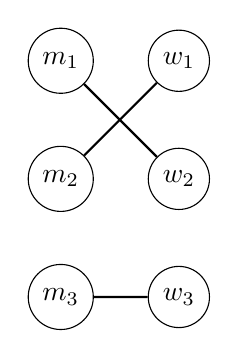
\begin{tikzpicture}[scale=1.5]
    % Draw nodes for men
    \node[circle, draw] (1) at (0, 1) {$m_1$};
    \node[circle, draw] (2) at (0, 0) {$m_2$};
    \node[circle, draw] (3) at (0, -1) {$m_3$};

    % Draw nodes for women
    \node[circle, draw] (4) at (1, 1) {$w_1$};
    \node[circle, draw] (5) at (1, 0) {$w_2$};
    \node[circle, draw] (6) at (1, -1) {$w_3$};

    % Draw edges representing the stable matching
    \draw[thick] (1) -- (5);
    \draw[thick] (2) -- (4);
    \draw[thick] (3) -- (6);
\end{tikzpicture}
\end{center}

\begin{center}
    \textbf{Stable Matching Example}
\end{center}

To illustrate the Gale-Shapley algorithm, we start with $m_1$ and perform the $m$-optimal Gale-Shapley algorithm, where each man proposes to their most preferred woman who hasn’t yet rejected them. This process yields the stable matching: \( \{(m_1, w_2), (m_2, w_1), (m_3, w_3)\} \), which is computed in polynomial time.

\paragraph{Runtime Complexity}
In this classical form of the problem, the worst-case complexity is $O(n^2)$, where $n$ is the number of men and also women. This arises from the necessity to check each individual's preferences and potential matches. \cite{gusfield}

\paragraph{Pre-Survey Remarks}
The Stable Marriage Problem is tied closely to concepts in computational complexity, particularly when considering extensions or variations of the problem that can grow in computational complexity. The original problem serves as an illustration of the divide between problems that can be solved efficiently and those that are computationally difficult, NP-hard or NP-complete. 

While the classic stable marriage problem with the Gale-Shapley algorithm can be solved in polynomial time, many of its variations, such as finding a stable matching under additional constraints, mentioned in latter portions regarding ties in preferences, incomplete preference lists, can grow to be NP-complete and/or NP-hard.

Another notable variant, the Stable Roommates Problem\cite{gusfield}, seeks to find a stable matching among a single group of individuals, without predefined pairings. In this scenario, stability is not guaranteed, and finding a matching can become computationally challenging, particularly with extensions that push it into NP-complete computational complexity.

These complexities illustrate how adding real-world constraints can dramatically alter the computational complexity, pushing problems into more complex realms. This highlights the importance of studying these problems as a means to produce equitable outcomes for all individuals. 

\section*{Problem Survey}
This section explores the various types of problems and algorithms presented in the book and recent literature in order to assess the progress made on these topics in subsequent research.

\paragraph{Extended Gale-Shapley Algorithm}

The \emph{Extended Gale-Shapley Algorithm}, developed by Robert Irving and Dan Gusfield, refines the classic Gale-Shapley algorithm to address the stable marriage problem while accommodating complexities such as ties in preferences and incomplete preference lists. This algorithm allows for equal rankings among choices, where an agent may rank two agents equally, thus reflecting indifference, and handles scenarios where participants may not rank all members of the opposite group. The algorithm also maintains the order of preferences and resolves ties consistently, often using secondary criteria to break ties. Furthermore, the algorithm has practical applications in various fields, including medical residency matching, school assignments, and job recruitment, enhancing its use in realistic scenarios where preferences are not always defined.

This extension helps address scenarios with unequal sets and considers preferences that include indifference or unacceptable partners, leading to a more nuanced approach to finding stable matchings. \cite{gusfield}

\paragraph{Irving Stable Roommates Algorithm}
This algorithm provides a framework for solving the Stable Roommates Problem, allowing for a stable matching among a single group without predefined pairings. It introduces additional complexity in finding and verifying stable matches.
\cite{gusfield}

This problem's importance is evident as the system is still used today and will be for the foreseeable future. While not as crucial as relationship matching or kidney exchanges, colleges continue to look for ways to maximize satisfaction among students and their roommates.

\paragraph{Hospital and Resident Problem}
An application of the Stable Marriage framework, this problem addresses the allocation of medical residents to hospitals based on mutual preferences. It extends the original problem to allow for multiple residents being mapped to  single hospital, showcasing practical implications and the need for variation of the original problem. 

Furthermore, the Gale-Shapley algorithm is crucial in medical residency matching through the National Resident Matching Program (NRMP) in the United States. By efficiently pairing medical graduates with residency programs. While not the most equitable, this system can help minimize dissatisfaction and turnover among residents and programs and also seems to enhance the overall quality of medical training.
\cite{gusfield}

\paragraph{Equitable Stable Marriage Problem}
The \emph{equitable stable marriage problem} aims to minimize the maximum regret across all participants in the matching. In this version, the goal is to find a stable matching that spreads dissatisfaction evenly, ensuring that no single participant feels disproportionately worse off than the others. The aim is to make the most dissatisfied person's outcome as favorable as possible, reducing the overall disparity in dissatisfaction among participants.

The paper from Giannakopoulos et. al\cite{equitable} introduces an approach to the Equitable Stable Marriage Problem (ESMP), which was a problem initially proposed by Gusfield and Irving. The ESMP is computationally more complex and considered NP-hard. This makes finding an optimal solution efficiently highly unlikely and calls for the use of either a heuristic or approximation algorithms. Previous approximation algorithms and heuristics, have encountered limitations, particularly in terms of non-termination or impractical runtimes when applied to large datasets. The new method focuses on minimizing the gap between men’s and women’s sum-of-rankings of their spouses while still ensuring stability.

When comparing this approach with the original SMP, several key differences emerge. The Gale-Shapley algorithm, while ensuring a stable solution, tends to favor the proposing side, resulting in biased outcomes. The ESMP, on the other hand, seeks to reduce this bias by achieving equitable matchings, minimizing the difference in rankings between the two sides. Although the ESMP is NP-hard and thus more complex than the SMP. Additionally, the original SMP focuses solely on stability, without consideration for fairness, while the ESMP aims to optimize both stability and equity, ensuring that both sides have more balanced satisfaction levels in the match. In practical terms, the original SMP is straightforward to implement and guarantees termination with a stable solution, while prior solutions for the ESMP, such as Swing, have struggled with efficiency.

The algorithm from Giannakopoulos et. al\cite{equitable} is shown below.

\paragraph{Equitable Stable Marriage Algorithm:}
This algorithm seeks to find a stable matching between two groups where no one has disproportionate dissatisfaction with their match. It works by having individuals propose and evaluate potential partners in each iteration, trying to balance the regret between participants.

\paragraph{Main Steps}

\paragraph{Proposal Evaluation}
When someone receives a proposal, they compare it to their current partner:
\begin{itemize}
    \item If the proposer is better than their current partner, they break up with their old partner and accept the new one.
    \item If the proposer is not better, they reject the proposal.
    \item If a person accepts the new proposer, they also check if they can slightly improve their future choices (adjusting their satisfaction threshold for better partners).
\end{itemize}

\paragraph{Making Proposals}
A proposer makes an offer to the next person on their list:
\begin{itemize}
    \item If their current partner is not their best option, they propose to the next person.
    \item If the proposal is accepted, they get engaged to the new partner and break up with the old one.
    \item If rejected, they move on to the next option.
\end{itemize}

\paragraph{Iterative Case}
The algorithm runs in rounds:
\begin{itemize}
    \item In each round, an agent from a group/set is chosen to make proposals, either group A or group B, depending on a mathematical rule involving sine function. The oscillating function allows for randomness when selecting proposers and not simply choosing one group/set of agents as done in the original SMP.
    \item Every person in the chosen group proposes to someone, and this continues until no one wants to change their current match.
\end{itemize}

\paragraph{Termination Case}
The algorithm stops when everyone is content with their current match, no more proposals or breakups are happening. At this point, the solution is stable and equitable. Although, the authors have noted issues with their termination cases.

\paragraph{Description}
The algorithm works by having people from two groups propose to one another, aiming to minimize the worst-case dissatisfaction for anyone. People take turns proposing, and they will keep switching partners until they find someone who makes them happy enough that they stop looking for someone better. The process continues until no one wants to switch partners anymore, resulting in a stable and fair outcome for both groups. By alternating the group that proposes in each round, the algorithm grows in complexity but also ensures fairness in the matching process. 

\paragraph{Egalitarian Stable Marriage Problem}
Similar to the previous problem, the \emph{egalitarian stable marriage problem} seeks to minimize the total sum of the participants' ranks of their assigned partners. In this formulation, each individual ranks their possible partners in order of preference, and the objective is to find a stable matching that produces the lowest possible total rank sum, thus maximizing collective satisfaction. This version of the problem emphasizes fairness at a societal level, ensuring that as many participants as possible get partners they prefer higher on their lists.

The problem is also categorized as NP-hard and has several usable heuristics and approximation algorithms. Many of the algorithms make use of rotation partially ordered sets (rotation posets). The rotation posets can be used to find all stable matching of the problem and then find the optimal solution. The rotations occur until the change becomes the desired change in egalitarian costs or decreases. This draws inspiration from the Gusfield and Irving's Minimum Egalitarian Stable Marriage Problem\cite{gusfield}.

An algorithm that solves the Egalitrian SMP usually involves rotation posets \cite{mcdermid}. The following is a high level description of an algorithm from Siyuan Wu et. al \cite{wu}.

\paragraph{Egalitarian Stable Marriage Algorithm:}

\paragraph{How the Algorithm Works}

\begin{enumerate}
    \item \textbf{Initial Stable Matching (Gale-Shapley)}: 
    \begin{itemize}
        \item The algorithm begins by finding any stable matching using a basic stable marriage algorithm (the Gale-Shapley algorithm).
        \item This provides a starting point for further refinement, but it is not necessarily the most egalitarian.
    \end{itemize}
    
    \item \textbf{Identifying Rotations}:
    \begin{itemize}
        \item Once a stable matching is found, the algorithm identifies all rotations. A rotation represents a set of men and women who could essentially "swap" partners in a way that makes at least one of them happier without violating stability.
        \item Each rotation consists of a sequence of matched pairs, where each man can improve his match by switching to another woman in the rotation.
    \end{itemize}
    
    \item \textbf{Rotation Poset Construction}:
    \begin{itemize}
        \item The rotations identified form a poset, partially ordered set. Some rotations depend on others, meaning you cannot apply one rotation until another has been performed.
        \item This structure ensures that the algorithm respects dependencies when performing rotations, preventing any conflicts in stability.
    \end{itemize}
    
    \item \textbf{Applying Rotations}:
    \begin{itemize}
        \item The algorithm traverses the rotation poset, removing rotations that reduce the total dissatisfaction. By applying a rotation, some individuals get matched with partners they prefer over their current ones.
        \item The algorithm continues applying rotations in the correct order to reduce the overall dissatisfaction incrementally.
    \end{itemize}
    
    \item \textbf{Termination}:
    \begin{itemize}
        \item The algorithm stops when no further rotations can improve the total dissatisfaction. At this point, the matching is both stable and as close to egalitarian as possible, given the constraints of stability.
    \end{itemize}
\end{enumerate}

\paragraph{Simplified Example}

\textbf{Initial Gale-Shapley Matching}: Let’s say a set of men and women are paired based on the male optimal Gale-Shapley algorithm. This produces a stable matching but not necessarily the most balanced in terms of satisfaction.

\textbf{Identifying a Rotation}: The algorithm detects a set of men and women who can improve their partners by rotating. For instance, man A prefers woman X, currently paired with man B, and man B prefers woman Y, currently paired with man C. The rotation allows them to switch partners without destabilizing the matching.

\textbf{Rotation Poset}: If man A’s improvement depends on another rotation involving man D and woman Z, the algorithm must first resolve that rotation before allowing A’s rotation to proceed. 

\paragraph{Summary of the Algorithm}

\begin{enumerate}
    \item Find a stable matching using the Gale-Shapley algorithm.
    \item Identify all possible rotations, which are sequences of pair swaps that can improve dissatisfaction without introducing instability.
    \item Construct a rotation poset to manage the dependencies between different rotations.
    \item Apply rotations in the correct order to iteratively reduce total dissatisfaction.
    \item Stop when no more rotations can be applied, resulting in an egalitarian stable matching.
\end{enumerate}

\paragraph{Sex-Equal Stable Marriage Problem}
The \emph{sex equal stable marriage problem} focuses on achieving a balanced outcome for both groups. It aims to minimize the difference in average satisfaction between the two groups. In other words, the goal is to find a stable matching where the average ranks of assigned partners are as equal as possible between the two groups of agents. This problem ensures that neither group, on average, ends up significantly better off than the other. 

Similar to the Egalitarian Stable Marriage Problem, it can also be done using rotation posets, as done by Kazuo et. al\cite{equalstable}.

\paragraph{Rotation Poset Algorithm for the Sex Equal Stable Marriage Problem: }

The algorithm seeks to find a sex-equal stable matching by minimizing the dissatisfaction between participants from two groups while maintaining stability. The steps of the algorithm are as follows:

\begin{enumerate}
    \item \textbf{Rotation Poset Construction:} \\
    The algorithm constructs a rotation poset, which captures the dependencies between different rotations, sets of pair swaps that can improve dissatisfaction. The poset ensures that rotations are applied in a valid order, preserving stability.

    \item \textbf{Initialize Best Matching:} \\
    The algorithm initializes a variable $M_b$ (M-best) to store the best matching found during the process.
    
    \item \textbf{Partition Rotations:} \\
    Rotations are divided into two sets:
    \begin{itemize}
        \item \( R_L \): Rotations with dissatisfaction greater than a threshold \( \delta \) (predefined threshold of dissatisfaction, depends on strictness desired).
        \item \( R_S \): Rotations with dissatisfaction less than or equal to \( \delta \).
    \end{itemize}
    
    \item \textbf{Iterate Over Subsets of \( R_L \):} \\
    For each subset \( R \) of rotations in \( R_L \), the algorithm computes an \emph{egalitarian matching} that minimizes dissatisfaction.

    \item \textbf{Apply Rotations in Order:} \\
    The algorithm applies or removes rotations based on the order in the poset, ensuring that dissatisfaction stays within bounds and stability is maintained.

    \item \textbf{Update Best Matching:} \\
    If a better matching is found, $M_b$ is updated.
    
    \item \textbf{Termination:} \\
    The algorithm terminates by outputting $M_b$ if a valid matching is found, or "None" if no such matching exists.
\end{enumerate}

\paragraph{Man-Exchange Problem}

\paragraph{Background}
The \emph{Man-Exchange problem} is a variant of the stable marriage problem where multiple partners can be matched, and exchanges between them occur. The goal is to create a stable matching where no pair prefers each other over their current partners. This problem extends the traditional stable marriage problem by introducing more flexibility in partner preferences and matching, which leads to more complex stability conditions. \cite{survey}

\paragraph{Time Complexity}
The time complexity of solving the Man-Exchange problem depends on the specific approach taken. For a Gale-Shapley-inspired solution, the algorithm runs in \(\mathcal{O}(n^2)\), where \(n\) is the number of agents. However, the complexity can increase if additional constraints or exchanges are introduced.

\paragraph{Possible Algorithms}
\begin{itemize}
    \item \textbf{Gale-Shapley Algorithm (adapted)}: This is an adaptation of the classical Gale-Shapley algorithm for stable marriages, extended to allow multiple partners and exchanges between them. The algorithm iteratively proposes matches and eliminates unstable pairs. \cite{gusfield}
\end{itemize}

\paragraph{Many-to-Many Matching Problem}

\paragraph{Background}
The \emph{Many-to-Many Matching problem} generalizes the stable marriage problem to allow agents on both sides to be matched to multiple counterparts. This situation often arises in real-world markets, such as job matching where applicants can be matched to multiple companies, or school admissions where students can apply to multiple schools. Each agent has preferences over the potential matches, and the goal is to find a stable matching. \cite{survey}

\paragraph{Time Complexity}
An extension of the Gale-Shapley algorithm for many-to-many matchings has a time complexity of \(\mathcal{O}(n^2 \cdot k)\), where \(n\) is the number of agents and \(k\) represents the maximum number of potential matches per agent. \cite{survey}

\paragraph{Possible Algorithms}
\begin{itemize}
    \item \textbf{Extended Gale-Shapley Algorithm}: This algorithm extends the classic deferred acceptance approach to handle many-to-many matchings, ensuring that the resulting matching is stable. \cite{gusfield}
\end{itemize}

\paragraph{Student Project Allocation Problem (SPAP)}

\paragraph{Background}
The \emph{Student Project Allocation Problem} (SPAP) involves matching students to projects based on mutual preferences. Students have ranked preferences for projects, and projects may also have preferences for students (if advisors are involved). The aim is to find a stable matching where no student-project pair prefers each other over their current assignment. \cite{survey}

\paragraph{Time Complexity}
The time complexity of the SPAP depends on the constraints and preferences involved. In its simplest form, where the problem is a straightforward matching, the complexity is \(\mathcal{O}(n^2)\). However, the problem can become NP-hard when additional constraints, such as capacities or weights, are considered. \cite{survey}

\paragraph{Possible Algorithms}
\begin{itemize}
    \item \textbf{Gale-Shapley-based Matching}: A variant of the stable matching algorithm, adjusted to handle student-project allocations while maintaining stability in the assignments. \cite{gusfield}
\end{itemize} 

\paragraph{3D Stable Matching}

\paragraph{3D Stable Matching Keywords}
Below are essential keywords along with their definitions that are needed to understand the problem. \cite{3dstable}
\begin{itemize} 
\item \textbf{cyclical preferences:} In a 3D stable matching scenario, three types of agents each have ranked preferences over the other two types, forming cycles in the preference relationships. Each agent’s preferences are defined in relation to pairs of agents from the other two types, creating a cyclical preference structure, rather than a linear one, which complicates the matching process.
\item \textbf{blocking triple:} A set of three agents, one from each group, who prefer to be matched with each other over their current assignments. This concept is analogous to a \emph{blocking pair} in traditional two-sided matching, where an unmatched pair would both be better off if they were matched. In the 3D case, a blocking triple indicates instability, as it implies that at least three agents are dissatisfied with their current matching.

\item \textbf{strongly blocking triple:} A specific type of blocking triple where each agent in the triple strictly prefers to match with the other two members of the triple over their current assignments. This strict preference implies that if the matching were altered to include this triple, all three would be better off, signaling strong instability in the current matching.

\item \textbf{weakly blocking triple:} A blocking triple where at least one agent in the triple has an equal preference (indifference) between their current assignment and the proposed new match. In other words, one or more agents do not strictly prefer the new match but would still find it at least as favorable as their current assignment, making the matching weakly unstable.

\item \textbf{strongly stable matching:} A matching is considered strongly stable if no strongly blocking triples exist. In this case, there is no set of three agents who would all strictly prefer to be matched with each other over their current matches, thus ensuring a stronger form of stability in the matching.

\item \textbf{weakly stable matching:} A matching is weakly stable if there are no blocking triples of any kind—either strongly or weakly blocking. In a weakly stable matching, no trio of agents would prefer (or even be indifferent to) forming a different matching arrangement, leading to a minimal form of stability.

\end{itemize}

\paragraph{Background}
The \emph{3D stable matching problem} generalizes the two-sided matching problem to involve three distinct sets of agents. For instance, in a research collaboration scenario, students, projects, and advisors may all have preferences over each other. The objective is to find a stable matching among all three groups, which poses significant computational challenges. \cite{survey} \cite{3dstable}

\subsubsection*{3D Stable Matching Example}

This example shows preferences for each element in three groups \( A = \{a_1, a_2, a_3\} \), \( B = \{b_1, b_2, b_3\} \), and \( C = \{c_1, c_2, c_3\} \), demonstrating a cycle where each participant has preferences over pairs in the other two groups. Each table displays preferences in columns and rows, where each row shows the rank order of preferences.

\paragraph{Preferences of Set \( A \):}
\[
\begin{array}{|c|c|c|}
\hline
a_1 & a_2 & a_3 \\ \hline
b_2 \; c_3 & b_1 \; c_1 & b_3 \; c_2 \\ \hline
b_3 \; c_1 & b_2 \; c_3 & b_2 \; c_1 \\ \hline
b_1 \; c_2 & b_3 \; c_2 & b_1 \; c_3 \\ \hline
\end{array}
\]

\paragraph{Preferences of Set \( B \):}
\[
\begin{array}{|c|c|c|}
\hline
b_1 & b_2 & b_3 \\ \hline
c_2 \; a_1 & c_1 \; a_2 & c_3 \; a_3 \\ \hline
c_3 \; a_2 & c_2 \; a_3 & c_2 \; a_1 \\ \hline
c_2 \; a_3 & c_3 \; a_1 & c_1 \; a_2 \\ \hline
\end{array}
\]

\paragraph{Preferences of Set \( C \):}
\[
\begin{array}{|c|c|c|}
\hline
c_1 & c_2 & c_3 \\ \hline
a_2 \; b_1 & a_1 \; b_2 & a_3 \; b_3 \\ \hline
a_3 \; b_2 & a_2 \; b_3 & a_2 \; b_1 \\ \hline
a_2 \; b_3 & a_3 \; b_1 & a_1 \; b_2 \\ \hline
\end{array}
\]

\begin{center}
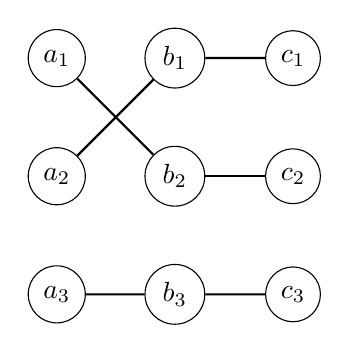
\begin{tikzpicture}[scale=1.5]

    \node[circle, draw] (1) at (0, 1) {$a_1$};
    \node[circle, draw] (2) at (0, 0) {$a_2$};
    \node[circle, draw] (3) at (0, -1) {$a_3$};

    \node[circle, draw] (4) at (1, 1) {$b_1$};
    \node[circle, draw] (5) at (1, 0) {$b_2$};
    \node[circle, draw] (6) at (1, -1) {$b_3$};

    \node[circle, draw] (7) at (2, 1) {$c_1$};
    \node[circle, draw] (8) at (2, 0) {$c_2$};
    \node[circle, draw] (9) at (2, -1) {$c_3$};

    \draw[thick] (1) -- (5); % $a_1 - b_2$
    \draw[thick] (2) -- (4); % $a_2 - b_1$
    \draw[thick] (3) -- (6); % $a_3 - b_3$

    \draw[thick] (4) -- (7); % $b_1 - c_1$
    \draw[thick] (5) -- (8); % $b_2 - c_2$
    \draw[thick] (6) -- (9); % $b_3 - c_3$
\end{tikzpicture}
\end{center}


\begin{center}
    3D Stable Matching Example
\end{center}

In the context of a 3D stable matching problem, each element in group \( A \) seeks a stable match with an element from group \( B \) and one from group \( C \). We start with the first iteration by examining the preferences of \( a_1 \). According to \( a_1 \)’s preference list, their top choice is the pair \( (b_2, c_3) \). To check compatibility, we look at \( b_2 \)'s preferences, which list \( (c_3, a_1) \) as an acceptable match, as a lower choice. Similarly, \( c_3 \) ranks \( (a_1, b_2) \) as their third choice, making the match mutually acceptable. This results in an initial match of \( (a_1, b_2, c_3) \). Using this approach for each individual’s top preferences, we complete the first round of matching with the triples \( (a_1, b_2, c_3) \), \( (a_2, b_1, c_1) \), and \( (a_3, b_3, c_2) \), which forms an initial stable matching configuration across groups.

\paragraph{Time Complexity}
The 3D stable matching problem is known to be NP-complete, making it computationally intractable for large inputs. Due to the involvement of three sets of agents, the search space becomes exponentially large, complicating the problem even further. \cite{survey}

\paragraph{Possible Algorithms}
\begin{itemize}
    \item \textbf{Approximation Algorithms}: Due to the NP-completeness of the problem, approximation algorithms are often used in practice to find near-optimal stable matchings in a more computationally feasible manner. \cite{gusfield}
    \item \textbf{Heuristic Algorithms}: Similarly, due to the NP-completeness of the problem, heuristic algorithms are used to find near-optimal stable matchings for 3D graphs. 
    \cite{3dstable}

    As it currently stands, there is no efficient algorithms for 3D Stable Matchings and thus requires further research.
\end{itemize}

\paragraph{One-Sided Preference Lists}

\paragraph{Background}
In the \emph{One-Sided Preference Lists problem}, only one side of the market has preferences, while the other side does not. This scenario can arise in markets where one set of participants, such as students, has preferences over options that do not rank them in return. The goal is to find a matching that is "popular," meaning no other matching would be preferred by a majority of the participants. \cite{survey}

\paragraph{Time Complexity}
The complexity of solving the One-Sided Preference Lists problem varies depending on the approach used, but it is often polynomial-time solvable for basic versions of the problem. \cite{gusfield}

\paragraph{Summary of Time Complexities}
\begin{table}[h!]
\centering
\begin{tabular}{|p{7cm}|c|}
\hline
\textbf{Problem} & \textbf{Time Complexity} \\
\hline
Stable Marriage Problem & \(\mathcal{O}(n^2)\) \\
Man-Exchange Problem & \(\mathcal{O}(n^2)\) \\
Many-to-Many Matching Problem & \(\mathcal{O}(n^2 \cdot k)\) \\
3D Stable Matching & NP-complete \\
One-Sided Preference Lists & \(\mathcal{O}(n^2)\) \\
Egalitarian Stable Marriage & NP-hard \\
Equitable Stable Marriage & NP-hard \\
Sex-Equal Stable Marriage & NP-hard \\
Stable Marriage Problem with Incomplete Preference Lists and Ties & NP-hard \\
\hline
\end{tabular}
\caption{Summary of Time Complexities for Matching Problems}
\end{table}

As stated earlier, we can see there is a lot of difference in complexity when comparing the original problem with its variants, highlighting that subtle changes and slightly different real-world applications greatly affect the runtime.

\section*{Real-World Application of Stable Marriage Problems}
While evidently important to the theoretical field of computer science and matching problems. It is also important to see how these algorithms are being used in contemporary society. Not only is it important to design these algorithms for equitable outcomes for all people but also to criticize when it is not being used as such. Thus, we will explore several applications in this section.

\paragraph{Modern Use of Gale-Shapley Algorithm} As stated in the paper "Testing How Dating Apps Recommend a Potential Matches for User", Soemardi et al. highlight how Tinder uses both the Gale-Shapley algorithm combined with the Elo Rating System introduced by Arpand Elo for the World Chess Federation. This has proved to be problematic as studies have shown that that the app, along with Bumble, lead to increased anxiety and problematic patterns of online dating use. \cite{calvin}

In his paper, "Are Tinder and Dating Apps Changing Dating and Mating in the USA?", Michael Rosenfield highlights how the increasing reliance on these apps that use the Gale-Shapley algorithm have become increasingly problematic via the larger problem of the effect of the Internet on social interaction. Despite the intention of both the algorithm and the dating apps to be create long lasting relationships for individuals, the overwhelming amount of data reveals that it leads to "hookups" and short-term relationships. It also seems to allow people to cycle through many different partners in a shorter period of time as they assume they can improve their compatibility with a partner despite not always being the case. \cite{Rosenfeld2018}

Outside of dating apps, the Gale-Shapley algorithm has been used in optimizing power allocation of 5G networks as seen in a paper "Optimizing 5G Power Allocation Communication: A Gale-Shapley Algorithm Approach" by Alruwaili et al. The algorithm increased total network capacity and also had good power amplitude relative to the other algorithms. While the algorithm increases overhead compared to simpler, previous algorithms, it could help future resource allocation and allow for more robust data transmission. \cite{10443942}

\section*{Conclusion}
In this section, we have explored the stable marriage problem and some if its variants. The use of these problems emphasize the importance of ensuring equitable outcomes for all people. For more information on these types of problems, readers may refer to the references, I recommend starting with the textbook, \emph{The Stable Marriage Problem - Structure and Algorithms} by Dan Gusfield and Robert W. Irving.

%\printbibliography{}
\nocite{mcvitie}
\nocite{popmatch}
\nocite{RONN1990285}
\nocite{wiki}
